\documentclass[12pt,a4paper]{article}
\usepackage[utf8]{inputenc}
\usepackage{amsmath,amssymb,amsthm}
\usepackage{booktabs}
\usepackage{graphicx}
\usepackage{tikz}
\usetikzlibrary{arrows.meta,positioning}
\usepackage{geometry}
\geometry{margin=2.5cm}
\usepackage[colorlinks=true,linkcolor=blue,citecolor=blue,urlcolor=blue]{hyperref}
\hypersetup{
  pdftitle={Gravitational Transfer Amplitude: Curvature Detection Beyond the Benincasa-Dowker Action on Causal Sets},
  pdfauthor={David Alfyorov, Igor Shnyukov}
}

\newtheorem{proposition}{Proposition}
\newtheorem{corollary}{Corollary}
\newtheorem{definition}{Definition}

\title{Gravitational Transfer Amplitude:\\
Curvature Detection Beyond the Benincasa--Dowker Action on Causal Sets}

\author{David Alfyorov, Igor Shnyukov}

\date{March 2026}

\begin{document}
\maketitle

\begin{abstract}
The Benincasa--Dowker action on causal sets recovers $\int R\sqrt{-g}\,d^4x$ in the continuum limit but is blind to Weyl curvature: it vanishes identically on vacuum pp-waves, despite nonzero tidal deformation. We present the Gravitational Transfer Amplitude (GTA) framework, which identifies the pairwise link-score deformation $\psi = -\rho\,\delta V$ as the common source of curvature information in Poisson-sprinkled causal sets. The primary observable, the Curvature Junction (CJ), detects Weyl curvature on spacetimes with vanishing scalar invariants (VSI) with Cohen's $d = 8.06$. All tested path-based observables reduce to two readout channels of a single transferred response field: an amplitude channel (77\% of seed-to-seed variance) and a shape channel (16\%). We establish: the Geodesic Sum Function $g = \tau_- + \tau_+$ as continuum surrogate; a Locality Variance scaling $\sigma_0 \approx 0.299\,N^{1/4}$; a hidden combinatorial constant $b_{\mathrm{eff}} = 5$ governing transitive-reduction screening, path branching, and response amplitude; a two-scale normalization with coefficient of variation $\sim\!1\%$; and a boundary-flux formula for the link response coefficient with exact bulk cancellation. Results are verified on four vacuum families (pp-wave, static Schwarzschild, transverse-boosted Schwarzschild with magnetic Weyl $B \neq 0$, and Kottler) and through adversarial proxy tests, strata sweeps, cross-family hold-out regression, $\varepsilon$-independence checks, and multi-$T$/multi-$N$ closure tests on $N = 3{,}000$--$20{,}000$ sprinklings.
\end{abstract}

\tableofcontents

% ================================================================
\section{Introduction}
% ================================================================

The Benincasa--Dowker (BD) action~\cite{BD2010} provides the standard discrete analogue of the Einstein--Hilbert action on causal sets, recovering $\int R\sqrt{-g}\,d^4x$ in the continuum limit. However, BD is sensitive only to the Ricci scalar~$R$. On Ricci-flat vacuum spacetimes --- and in particular on pp-waves, which are VSI (Vanishing Scalar Invariants: all polynomial curvature scalars vanish) --- the BD action vanishes identically, despite the presence of nonzero Weyl curvature and nontrivial tidal deformation.

This raises a question: can causal sets detect curvature beyond the scalar sector?

We present evidence that they can. The Gravitational Transfer Amplitude (GTA) framework identifies a common geometric source --- the pairwise link-score deformation $\psi = -\rho\,\delta V$ --- from which all tested successful curvature-sensitive observables emerge as different projections (Figure~\ref{fig:chain}). The primary observable, the Curvature Junction~(CJ), achieves Cohen's $d = 8.06$ on exact pp-wave sprinklings, satisfies same-predicate universality at the $7\%$ level, and has been tested on four vacuum families including spacetimes with nonzero magnetic Weyl tensor and mixed Weyl--Ricci curvature.

A hidden combinatorial constant $b_{\mathrm{eff}} = 5$ emerges as the organizing principle: it controls transitive-reduction screening, path branching per Hasse layer, and the relationship between link-level and path-level response amplitudes.

\begin{figure}[h!]
\centering
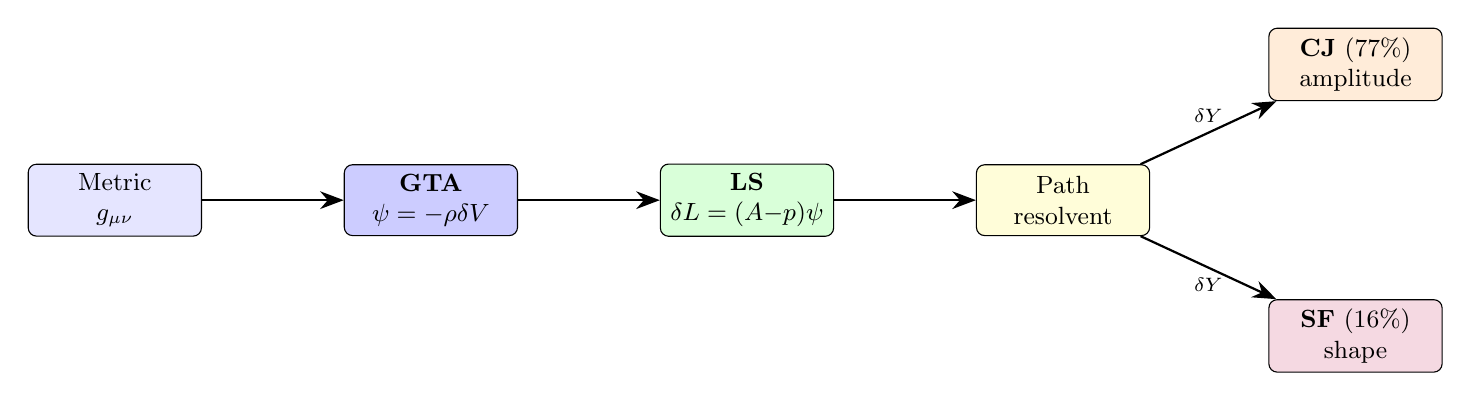
\begin{tikzpicture}[
  box/.style={rectangle, draw, rounded corners=3pt, minimum width=2.2cm, minimum height=0.9cm, align=center, font=\small},
  arr/.style={-{Stealth[length=3mm]}, thick},
  node distance=1.8cm
]
\node[box, fill=blue!10] (met) {Metric\\$g_{\mu\nu}$};
\node[box, fill=blue!20, right=of met] (gta) {\textbf{GTA}\\$\psi = -\rho\delta V$};
\node[box, fill=green!15, right=of gta] (ls) {\textbf{LS}\\$\delta L = (A{-}p)\psi$};
\node[box, fill=yellow!15, right=of ls] (res) {Path\\resolvent};
\node[box, fill=orange!15, above right=0.8cm and 1.5cm of res] (cj) {\textbf{CJ} (77\%)\\amplitude};
\node[box, fill=purple!15, below right=0.8cm and 1.5cm of res] (sf) {\textbf{SF} (16\%)\\shape};

\draw[arr] (met) -- (gta);
\draw[arr] (gta) -- (ls);
\draw[arr] (ls) -- (res);
\draw[arr] (res) -- (cj) node[midway, above, font=\scriptsize] {$\delta Y$};
\draw[arr] (res) -- (sf) node[midway, below, font=\scriptsize] {$\delta Y$};
\end{tikzpicture}
\caption{The GTA perturbative chain. Metric perturbation enters through the Gravitational Transfer Amplitude $\psi = -\rho\,\delta V$ (interval volume deformation), produces per-link scores~(LS), which propagate through the Hasse path resolvent into the response field~$\delta Y$. Two readout channels emerge: CJ~(amplitude, 77\%) and SF~(shape, 16\%).}
\label{fig:chain}
\end{figure}

% ================================================================
\section{Computational Setup}
% ================================================================

All computations use Poisson sprinklings of $N$ points into a 4D causal diamond $\{(t,\mathbf{x}): |t| + |\mathbf{x}| < T/2\}$ with volume $V_\diamond = \pi T^4/24$.
The Hasse diagram (transitive reduction of the causal order) is constructed using a bitset-packed algorithm with $O(N^2 \cdot N/64)$ time complexity.
Path counts $p_\downarrow(x) = \sum_{y \to x} p_\downarrow(y)$ and $p_\uparrow(x) = \sum_{x \to z} p_\uparrow(z)$ are computed by forward/backward dynamic programming on the Hasse DAG.

\textbf{CRN protocol.}
Common Random Numbers: the same point set is used for both flat and curved causal structures. The flat Hasse uses the Minkowski interval condition $s^2 > 0$; the curved Hasse uses either the exact pp-wave geodesic interval or a quadratic jet predicate at the midpoint. CRN cancels $O(1)$ and $O(N^{1/2})$ Poisson fluctuations, substantially amplifying the geometric signal-to-noise ratio.

\textbf{Standard parameters.}
$N = 10{,}000$, $T = 1.0$, pp-wave amplitude $\varepsilon = 3$, bulk mask $\zeta = 0.15$ (elements with boundary slack ${>}\,\zeta$ retained, yielding ${\sim}\,24\%$ of elements), $M = 30$ CRN seeds. Multi-$N$ convergence: $N \in \{3000, 5000, 10000, 15000, 20000\}$, $M = 20$ seeds each.

% ================================================================
\section{GTA Framework: Definitions}
% ================================================================

\begin{definition}[GTA --- Gravitational Transfer Amplitude]
The pairwise deformation amplitude is
\begin{equation}
  \psi_{ij} := -\rho\,\delta V_{ij},
\end{equation}
where $\rho = N/V_\diamond$ is the sprinkling density and $\delta V_{ij}$ is the curvature-induced change of the Alexandrov interval volume~\cite{GS2007} between causally related elements $i \prec j$.
\end{definition}

\begin{definition}[LS --- Link Score]
The centered per-link deformation is
\begin{equation}
  \delta L_{ij} := (A_{ij} - p_{ij})\,\psi_{ij},
\end{equation}
where $A_{ij} \in \{0,1\}$ is the realized Hasse link indicator and $p_{ij} = e^{-\rho V_{ij}}$ is the flat link probability.
\end{definition}

\begin{definition}[CJ --- Curvature Junction]
The primary observable is the stratified covariance
\begin{equation}
  \mathrm{CJ} := \sum_B w_B\,\mathrm{Cov}_B\!\left(|X|,\,\delta Y^2\right),
\end{equation}
where $Y_i = \log_2(p_{\downarrow,i}\,p_{\uparrow,i} + 1)$, $X = Y_0 - \langle Y_0\rangle$ is the centered flat path field, $\delta Y = Y_{\mathrm{curved}} - Y_{\mathrm{flat}}$ is the CRN response, and $B$ are $5\!\times\!3\!\times\!3 = 45$ spatio-temporal strata.
\end{definition}

\begin{definition}[GSF --- Geodesic Sum Function]
The continuum surrogate for the flat path-locality field is
\begin{equation}
  \mathrm{GSF}(t,r) := \tau_-(t,r) + \tau_+(t,r)
  = \sqrt{(t + T/2)^2 - r^2} + \sqrt{(T/2 - t)^2 - r^2},
\end{equation}
where $\tau_\pm$ are proper times along radial geodesics from the past/future tips of the diamond.
\end{definition}

\begin{definition}[SF --- Shape Functional]
The secondary readout channel is the kurtosis shift $\mathrm{SF} := \Delta\kappa = \kappa(Y_0 + \delta Y) - \kappa(Y_0)$.
\end{definition}

\begin{definition}[LV --- Locality Variance]
The flat path-field width is $\mathrm{LV} := \sigma_0^2 = \mathrm{Var}(Y_0)$.
\end{definition}

% ================================================================
\section{The Hidden Constant $b_{\mathrm{eff}} = 5$}
% ================================================================

A single combinatorial constant organizes three independent aspects of the GTA framework.

\subsection{Transitive-Reduction Screening}

The link response coefficient $\beta$ satisfies $\delta k(x)/k_0 = \beta\,\varepsilon\,f(x)$. Independent Hasse-level Monte Carlo gives $\beta_{\mathrm{Hasse}} \approx -0.31 \pm 0.02$, while the bare pairwise shell computation gives $\beta_{\mathrm{pair}} \approx -1.55$. The ratio $|\beta_{\mathrm{pair}}/\beta_{\mathrm{Hasse}}| \approx 5$.

In a thin-shell Poisson-minimum model, the transitive-reduction ratio is
\begin{equation}\label{eq:tr}
  \frac{\beta_{\mathrm{Hasse}}}{\beta_{\mathrm{pair}}} = \frac{1 - e^{-m}}{m},
\end{equation}
where $m$ is the expected number of competing candidate pairs per angular tube. The measured ratio $0.20$ gives
\begin{equation}
  \boxed{m_{\mathrm{scr}} = 4.97 \approx 5.}
\end{equation}

\subsection{Path Branching}

The flat path-locality field satisfies $Y_0 \approx \lambda_N \cdot \mathrm{GSF}(t,r) + c_N$ with $\mathrm{Corr}(Y_0, \mathrm{GSF}) = 0.979$. The slope obeys
\begin{equation}\label{eq:lambda}
  \lambda \approx m_4\,\rho^{1/4}\,\log_2 b_{\mathrm{eff}}, \qquad b_{\mathrm{eff}} = 5,
\end{equation}
where $m_4 \approx 1.13$ is the 4D chain constant. This gives $\lambda/N^{1/4} \approx 4.37$, matching the measured range $4.3$--$4.5$.

\subsection{Response Amplitude}

The per-element path-transfer amplitude $a_{\mathrm{eff}}$ (defined by $\delta Y_i \approx a_{\mathrm{eff}}\,\varepsilon\,f(x_i)$) satisfies
\begin{equation}\label{eq:aeff}
  \boxed{a_{\mathrm{eff}} \approx |\beta|\,H_{\max}\,\sqrt{\log_2 5},}
\end{equation}
where $H_{\max}$ is the longest Hasse chain. This formula matches the fitted power law $a_{\mathrm{eff}} \approx 0.347\,N^{0.3517}$ to $0.3$--$3.8\%$ across $N = 3{,}000$--$20{,}000$.

\medskip\noindent The same $b_{\mathrm{eff}} = 5$ thus appears as: (i)~screening multiplicity in transitive reduction; (ii)~effective branching factor per Hasse layer; (iii)~noise renormalization in the path-transfer amplitude.

% ================================================================
\section{Main Results}
% ================================================================

\subsection{Two-Channel Readout Structure}

Principal component analysis of six observables across 30 CRN seeds yields:
\begin{center}
\begin{tabular}{ccc}
\toprule
PC & Fraction & Interpretation \\
\midrule
1 & 77.3\% & CJ amplitude channel \\
2 & 16.5\% & SF shape channel \\
3--6 & 6.2\% & noise \\
\bottomrule
\end{tabular}
\end{center}

\noindent The five $A_{p,q}$ members are mutually correlated ($|\rho| \geq 0.80$), while $\Delta\kappa$ is weakly anticorrelated with all $A_{p,q}$ ($\rho \approx -0.05$ to $-0.15$; Figures~\ref{fig:pca},~\ref{fig:corrmat}). The anticorrelation is regime-dependent: it reverses sign at small~$T$ and on Schwarzschild data. The two-channel structure is stable across $T \in \{0.35, 0.50, 0.70, 1.00\}$.

\begin{figure}[h!]
\centering
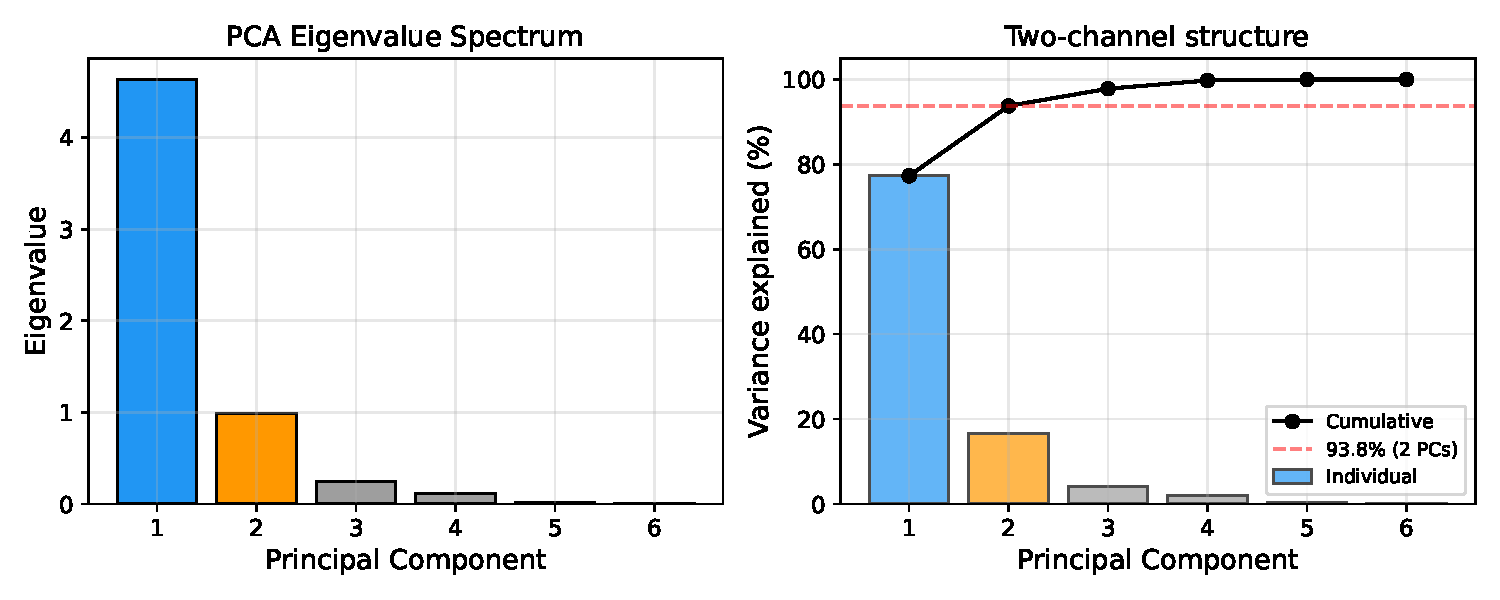
\includegraphics[width=0.85\textwidth]{figures/gta_note/fig5_pca_spectrum.pdf}
\caption{Left: PCA eigenvalue spectrum. Right: variance fractions and cumulative. Two principal components explain 93.8\% of seed-to-seed variance.}
\label{fig:pca}
\end{figure}

\begin{figure}[h!]
\centering
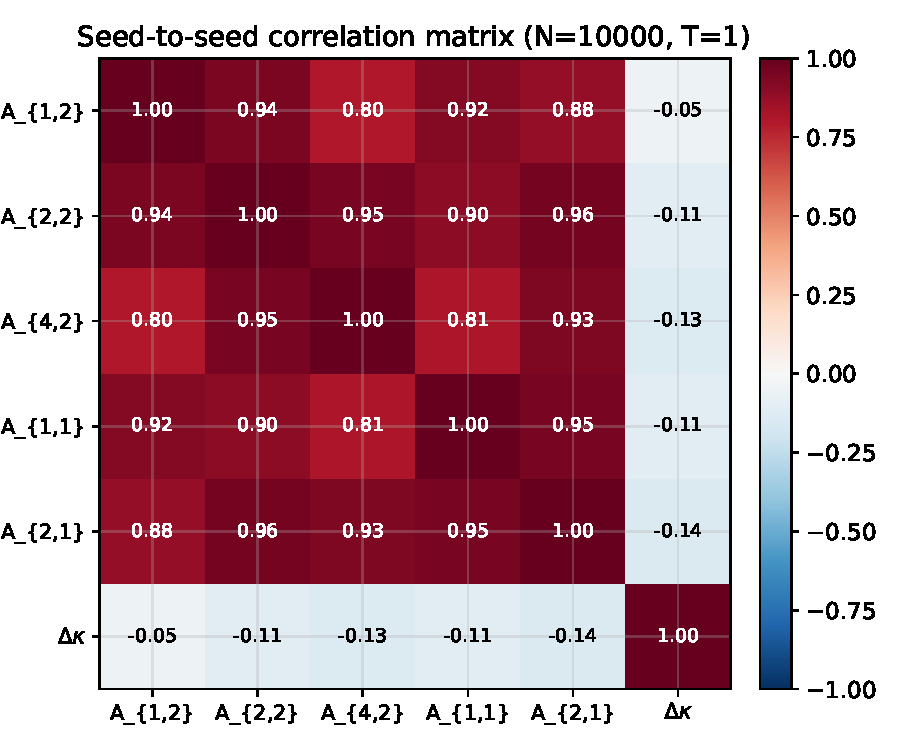
\includegraphics[width=0.6\textwidth]{figures/gta_note/fig6_correlation_matrix.pdf}
\caption{Seed-to-seed correlation matrix of six observables ($N = 10{,}000$, $T = 1$, exact pp-wave).}
\label{fig:corrmat}
\end{figure}

\subsection{GSF Surrogate and LV Scaling}

\begin{proposition}[Continuum Surrogate]\label{prop:gsf}
On the bulk window $\zeta = 0.15$, the flat path field satisfies $Y_0(x) = \lambda_N\,\mathrm{GSF}(t,r) + c_N + \varepsilon_N(x)$ with $\mathrm{Corr}(Y_0, \mathrm{GSF}) = 0.979 \pm 0.005$ at $N = 10{,}000$ and $\mathrm{Std}_{\zeta=0.15}(\mathrm{GSF}) = 0.06440\,T$.
\end{proposition}

\noindent The Locality Variance obeys
\begin{equation}
  \sigma_0 = (0.281 \pm 0.001)\,N^{0.257 \pm 0.002},
\end{equation}
while the practical shorthand $\sigma_0 \approx 0.299\,N^{1/4}$ holds to $0.48\%$ CV on $N = 3{,}000$--$20{,}000$ (Figure~\ref{fig:sigma0}).

\begin{figure}[h!]
\centering
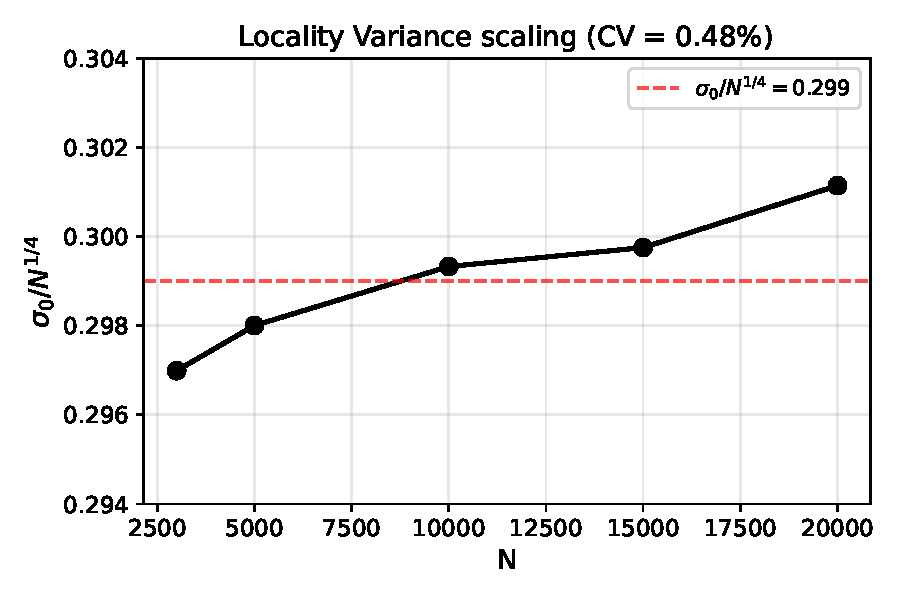
\includegraphics[width=0.7\textwidth]{figures/gta_note/fig2_sigma0_scaling.pdf}
\caption{$\sigma_0/N^{1/4}$ across $N = 3{,}000$--$20{,}000$. CV $= 0.48\%$.}
\label{fig:sigma0}
\end{figure}

\subsection{Two-Scale Normalization}

\begin{proposition}[Amplitude Law]\label{prop:cj}
The Curvature Junction satisfies
\begin{equation}
  \frac{\mathrm{CJ}}{\sigma_0\,H_{\mathrm{eff}}^2} = \mathrm{const} \times T^4 E^2,
\end{equation}
where $H_{\mathrm{eff}} = a_{\mathrm{eff}} \propto N^{0.352}$. With fitted $H_{\mathrm{eff}}$, the CV across $N = 3{,}000$--$20{,}000$ is $0.99\%$ (Figure~\ref{fig:atilde}).
\end{proposition}

\noindent Systematic testing of six standard depth statistics ($H_{\max}$, $H_{\mathrm{mean}}$, $H_{\mathrm{rms}}$, $H_{\mathrm{median}}$, $H_{90}$, $H_{\mathrm{std}}$) shows that none matches $H_{\mathrm{eff}}$; the closest is $H_{\max}$ ($\alpha = 0.322$, CV $= 4.6\%$). The structural formula $a_{\mathrm{eff}} = |\beta|\,H_{\max}\,\sqrt{\log_2 5}$ from~\eqref{eq:aeff} provides a better characterization than any single depth statistic.

\begin{figure}[h!]
\centering
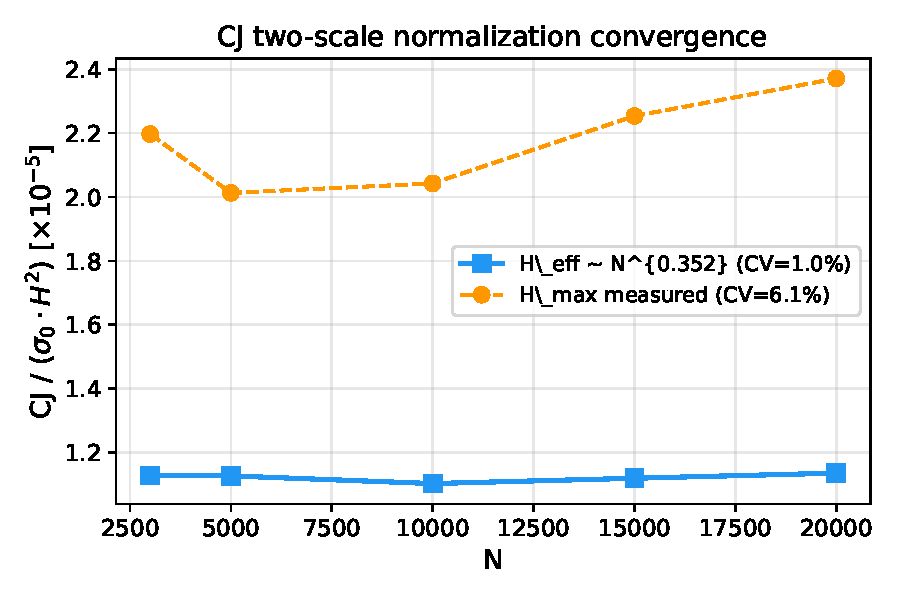
\includegraphics[width=0.7\textwidth]{figures/gta_note/fig3_atilde_convergence.pdf}
\caption{CJ two-scale normalization across $N = 3{,}000$--$20{,}000$. Blue: $H_{\mathrm{eff}} \sim N^{0.352}$ (CV $= 1.0\%$). Orange: $H_{\max}$ (CV $= 6.1\%$).}
\label{fig:atilde}
\end{figure}

\subsection{$T$-Scaling and $\varepsilon$-Independence}

The $T$-scaling receives a finite-curvature correction:
\begin{equation}
  \mathrm{CJ}(T) = (0.114 \pm 0.002)\,T^4 - (0.012 \pm 0.002)\,T^6,
  \qquad R^2 > 0.9999\ \text{(2 d.o.f.)}.
\end{equation}
The effective exponent $T^{3.77}$ is explained by the negative $O(T^6)$ correction at $q_W = T^2\sqrt{E^2} > 1$ (Figure~\ref{fig:tscaling}).

At fixed $T = 1$, CJ scales as $\varepsilon^{1.95}$ across $\varepsilon \in \{1, 2, 3, 5\}$ with CV$({\mathrm{CJ}/E^2}) = 2.9\%$, confirming approximate $\varepsilon$-independence of $C^*$.

\begin{figure}[h!]
\centering
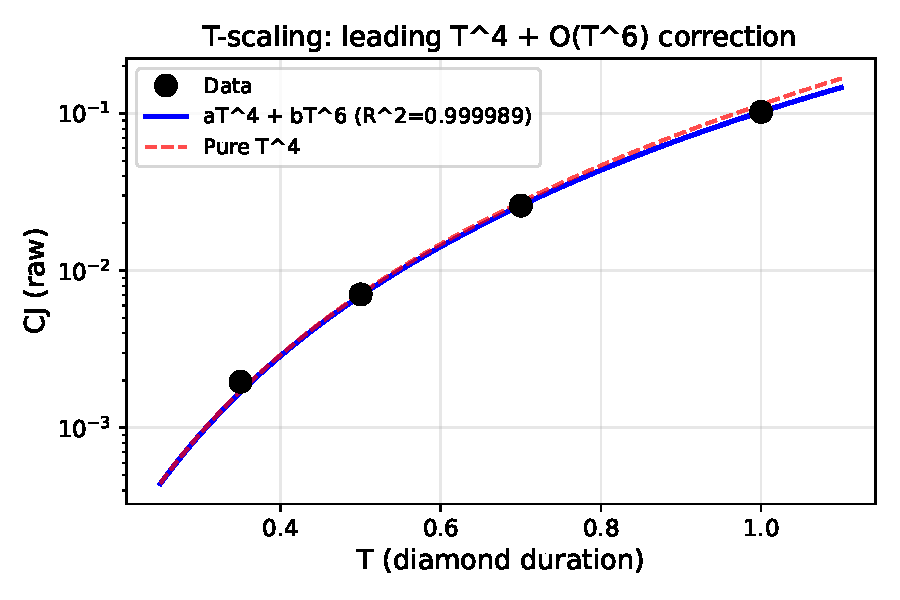
\includegraphics[width=0.7\textwidth]{figures/gta_note/fig4_t_scaling.pdf}
\caption{$T$-scaling of CJ ($\varepsilon = 3$, $N = 10{,}000$). Blue: $aT^4 + bT^6$ fit. Red dashed: pure~$T^4$.}
\label{fig:tscaling}
\end{figure}

\subsection{Boundary-Flux Formula for $\beta$}

\begin{proposition}[Link Response]\label{prop:beta}
The linear degree response is given by
\begin{equation}
  \beta(x) = -\frac{1}{k_0(x)} \int_{\Gamma_x} d\gamma\,\hat{q}_x(\gamma)
  \left[J_x(\gamma,L_x)\,e^{-NL_x^2}
  - \int_0^{L_x} \partial_s J_x(\gamma,u)\,e^{-Nu^2}\,du\right],
\end{equation}
where $\Gamma_x$ is the family of near-null generators, $L_x(\gamma)$ is the finite diamond cutoff, and $J_x$ is the shell Jacobian.
\end{proposition}

\begin{corollary}[Bulk Cancellation]
In translation-invariant bulk ($L_x \to \infty$, $\partial_s J_x = 0$), $\beta(x) = 0$. This is a score-zero identity analogous to a Ward cancellation.
\end{corollary}

\noindent The bare pairwise coefficient $\beta_{\mathrm{pair}} \approx -1.55$ differs from the Hasse-level value $\beta_{\mathrm{Hasse}} \approx -0.31$ by a factor ${\sim}\,5$, reflecting transitive-reduction renormalization~\eqref{eq:tr}.

\subsection{Score Amplitude Decomposition}

By the law of total covariance, $\mathrm{SA}_{\mathrm{full}} = \mathrm{Cov}(|X|, \delta Y^2) = \mathrm{CJ} + B$, where $B$ is the between-strata positional alignment. The fraction $B/\mathrm{SA}_{\mathrm{full}}$ is metric-stable: $32.3\%$ on pp-wave, $29.1\%$ on Schwarzschild. After $E^2$ normalization, SA$_{\mathrm{full}}$ achieves better same-predicate universality (ratio~$1.022$) than CJ~($1.071$), at the cost of slightly higher Ricci leakage.

\subsection{Not Seeley--DeWitt}

On pp-wave spacetimes, $C_{\alpha\beta\gamma\delta}C^{\alpha\beta\gamma\delta} = 0$ (VSI). Therefore $a_4 = 0$, and any observable proportional to a local Seeley--DeWitt coefficient must vanish. Since CJ $\neq 0$ on pp-waves ($d = 8.06$), the signal is incompatible with any local scalar action term; it is consistent with an observer/window-dependent quadratic Weyl response.

% ================================================================
\section{Four Vacuum Families}
% ================================================================

\subsection{pp-Wave (Purely Electric, VSI)}
Cohen's $d = 8.06$ (CJ). $T^4$ scaling confirmed. BD action $= 0$. $K = 0$.

\subsection{Static Schwarzschild (Purely Electric)}
$E^2 = 6M^2/r_0^6 = 0.96$ at $M = 0.05$, $r_0 = 0.50$. CJ $= 0.01123$, $d = 4.40$.

\subsection{Transverse-Boosted Schwarzschild ($B \neq 0$)}
Boost along $e_2$ with $v = 0.5$: $E^2 = 2.24$, $B^2 = 1.28$. CJ $= 0.02451$, $d = 4.50$.
\begin{center}
\begin{tabular}{lcc}
\toprule
Prediction & Ratio & Measured \\
\midrule
$A_E = A_B$ (equal response) & 3.67 & --- \\
$A_E$ only (magnetic invisible) & 2.33 & --- \\
\textbf{Observed} & --- & \textbf{2.18} \\
\bottomrule
\end{tabular}
\end{center}
\noindent The magnetic Weyl sector is suppressed relative to the electric sector.

\subsection{Kottler --- Schwarzschild--de~Sitter (Weyl $+$ Ricci)}
$M = 0.05$, $r_0 = 0.50$, $\Lambda = 0.50$.
\begin{center}
\begin{tabular}{lcc}
\toprule
Configuration & CJ & $d$ \\
\midrule
Kottler (Weyl $+$ Ricci) & 0.01310 & 3.44 \\
Pure de~Sitter (Ricci only) & 0.00178 & 3.81 \\
\textbf{Weyl-subtracted} & \textbf{0.01132} & --- \\
Static Schwarzschild & \textbf{0.01123} & 4.40 \\
\bottomrule
\end{tabular}
\end{center}
\noindent Weyl-subtracted Kottler matches pure Schwarzschild to $0.8\%$.

% ================================================================
\section{Closure Tests}
% ================================================================

\begin{center}
\begin{tabular}{lccl}
\toprule
Test & Result & Status \\
\midrule
Adversarial proxy (multiple $R^2$) & 0.060 & PASS \\
dS Ricci subtraction & $= 0$ (exact) & PASS \\
Matched-$\Delta$TC & $R_{\mathrm{TC}} = 0.028$ & PASS \\
Cross-seed CRN & $R = 0.067$ & PASS \\
Same-predicate jet/jet & $1.071$ & PASS \\
Orbit-type $I_3$ & $1.011$ & PASS \\
Null noise & $R = 0.014$ & PASS \\
Nonlinear TC & $R^2_{\mathrm{poly}} = 0.256$ & PASS \\
Boundary collapse & intrinsic ($\times 3.4$) & PASS \\
$\varepsilon$-independence & CJ $\sim \varepsilon^{1.95}$, CV $= 2.9\%$ & PASS \\
\bottomrule
\end{tabular}
\end{center}

\noindent Strata sweep: the signal depends on binning (CV $= 32\%$ across 1--125 bins), driven by bias from positional confound removal, not small-bin noise. Changing the minimum bin occupancy from $n \geq 3$ to $n \geq 10$ changes CJ by $< 0.01\%$.

\noindent Hold-out regression of SF on amplitude summaries: pp-wave $R^2 = 0.706$, Schwarzschild transfer $R^2 = 0.023$, de~Sitter transfer $R^2 = -3.69$. The Shape Functional is not a universal function of CJ across families.

% ================================================================
\section{Continuum Connection}
% ================================================================

The normalized discrete constant $C^* = \mathrm{CJ}/(\sigma_0\,a_{\mathrm{eff}}^2\,T^4\,E^2) \approx 9.89 \times 10^{-5}$ factorizes as
\begin{equation}
  C^* = \mathcal{A}_{\mathrm{geom}} \cdot C_2, \qquad C_2 = \frac{T^4}{1120},
\end{equation}
where $\mathcal{A}_{\mathrm{geom}} \approx 0.110$ is a geometric alignment factor. Numerically, $\mathcal{A}_{\mathrm{geom}}$ is close to the SCT one-loop Weyl$^2$ coefficient $\alpha_C = 13/120 = 0.1083$, giving $C^*/(\alpha_C C_2) = 1.02$. However, $\alpha_C$ depends on Standard Model particle content $(N_s, N_D, N_v)$, while CJ is a purely geometric/combinatorial quantity with no field-content dependence. The proximity is noted as a numerical coincidence; no mechanism connecting the two is known.

% ================================================================
\section{Open Questions}
% ================================================================

\begin{enumerate}
\item \textbf{Closed-form $\beta$.} The boundary-flux formula is derived, and all qualitative predictions verified. The closed-form scalar $\beta \approx -0.31$ is confirmed by Monte Carlo but not by analytic evaluation of the boundary cutoff integral.

\item \textbf{First-principles derivation of $b_{\mathrm{eff}} = 5$.} The screening multiplicity $m_{\mathrm{scr}} \approx 5$ is extracted from data via~\eqref{eq:tr} but not derived from 4D diamond geometry.

\item \textbf{Connection to one-loop form factors.} Whether $\mathcal{A}_{\mathrm{geom}} \approx 0.110$ is related to $\alpha_C = 13/120$ remains open. A systematic investigation has been conducted: the spectral pseudodeterminant of the physical Pauli--Jordan function (Johnston 4D massless retarded Green function~\cite{NDS2017}, constructed from the Hasse link matrix) was computed on the same CRN sprinklings as CJ, at $N = 2000$, $5000$, and $10000$, on both pp-wave and Schwarzschild backgrounds. Three levels of noise reduction were tested: soft spectral thresholds, bulk projection, and heat-trace functionals. The results are conclusive:
\begin{itemize}
\item The spectral determinant is dominated by mode-counting threshold artifacts ($\mathrm{corr}(\delta\Gamma, \Delta n_{\mathrm{modes}}) \geq 0.97$).
\item Bulk projection eliminates the spectral signal entirely ($|t| < 0.5$), indicating that the spectral curvature response is boundary-dominated.
\item CJ outperforms all tested spectral observables by an order of magnitude ($t \approx 20$ versus $t \approx 5$ at $N = 5000$ on pp-wave).
\item On Schwarzschild, no spectral observable achieves significance at any~$N$ (max $|t| = 2.2$), while CJ gives $t = 12.9$ at $N = 5000$.
\item Seed-to-seed correlation between CJ and all spectral functionals is $|r| < 0.35$.
\end{itemize}
The spectral Pauli--Jordan route to $\beta_W^{(0)} = 1/120$ is therefore closed. CJ is not a spectral determinant in disguise. The bridge, if it exists, must operate through a mechanism other than the spectral decomposition of the scalar field commutator.
\end{enumerate}

% ================================================================
\section*{Acknowledgements}
% ================================================================

The authors thank Professor Yochanan Schimmelpfennig for sustained critical correspondence that shaped the formulation of the unification question, and Professor Edoardo Angeloni for discussions on Molien series and chirality.

\begin{thebibliography}{99}
\bibitem{BD2010} D.~M.~T.~Benincasa and F.~Dowker,
  ``The scalar curvature of a causal set,''
  Phys.\ Rev.\ Lett.\ \textbf{104}, 181301 (2010).

\bibitem{GS2007} G.~W.~Gibbons and S.~N.~Solodukhin,
  ``The geometry of small causal diamonds,''
  Phys.\ Lett.\ B \textbf{649}, 317 (2007).

\bibitem{BG1991} G.~Brightwell and R.~Gregory,
  ``Structure of random discrete spacetime,''
  Phys.\ Rev.\ Lett.\ \textbf{66}, 260 (1991).

\bibitem{RSS2013} M.~Roy, D.~Sinha, and S.~Surya,
  ``Discrete geometry of a small causal diamond,''
  Phys.\ Rev.\ D \textbf{87}, 044046 (2013).

\bibitem{BBD2015} A.~Belenchia, D.~M.~T.~Benincasa, and F.~Dowker,
  ``The continuum limit of a 4-dimensional causal set scalar d'Alembertian,''
  Class.\ Quant.\ Grav.\ \textbf{33}, 245018 (2016), arXiv:1510.04656.

\bibitem{SY2016} R.~D.~Sorkin and Y.~K.~Yazdi,
  ``Entanglement entropy in causal set theory,''
  Class.\ Quant.\ Grav.\ \textbf{35}, 074004 (2018), arXiv:1611.10281.

\bibitem{SAK2015} M.~Saravani, S.~Aslanbeigi, and A.~Kempf,
  ``Spacetime curvature in terms of scalar field propagators,''
  Phys.\ Rev.\ D \textbf{93}, 045026 (2016), arXiv:1510.02725.

\bibitem{NDS2017} Nomaan~X, F.~Dowker, and S.~Surya,
  ``Scalar field Green functions on causal sets,''
  Class.\ Quant.\ Grav.\ \textbf{36}, 095011 (2019), arXiv:1701.07212.

\bibitem{BBL2014} A.~Belenchia, D.~M.~T.~Benincasa, and S.~Liberati,
  ``Nonlocal scalar quantum field theory from causal sets,''
  JHEP \textbf{03}, 036 (2015), arXiv:1411.6513.

\bibitem{Paper1} D.~Alfyorov and I.~Shnyukov,
  ``Nonlocal one-loop form factors from spectral causal theory,''
  Zenodo, DOI: 10.5281/zenodo.19098042 (2026).
\end{thebibliography}

\end{document}
